\chapter{Úniky způsobené vícecestným šířením}
Pro tento typ měření jsme potřebovali lokaci, kde bude velký pohyb chodců. Nejlépe takovou, aby docházelo k zastínění, ale také, aby zde ve vhodnou chvíli pohyb nebyl žádný nebo jen minimální. Nakonec jsme se rozhodli provést měření před vchodem do Technické menzy v Dejvicích. Čas měření nám velice vyhovoval, jelikož v tuto dobu - kolem 12. hodiny - je zde největší hustota lidí. Vzdálenost mezi anténami byla při měření 24 metrů a jednotlivé antény byly umístěny ve výšce 1,4 metru.

\begin{figure}[h!]
    \centering
    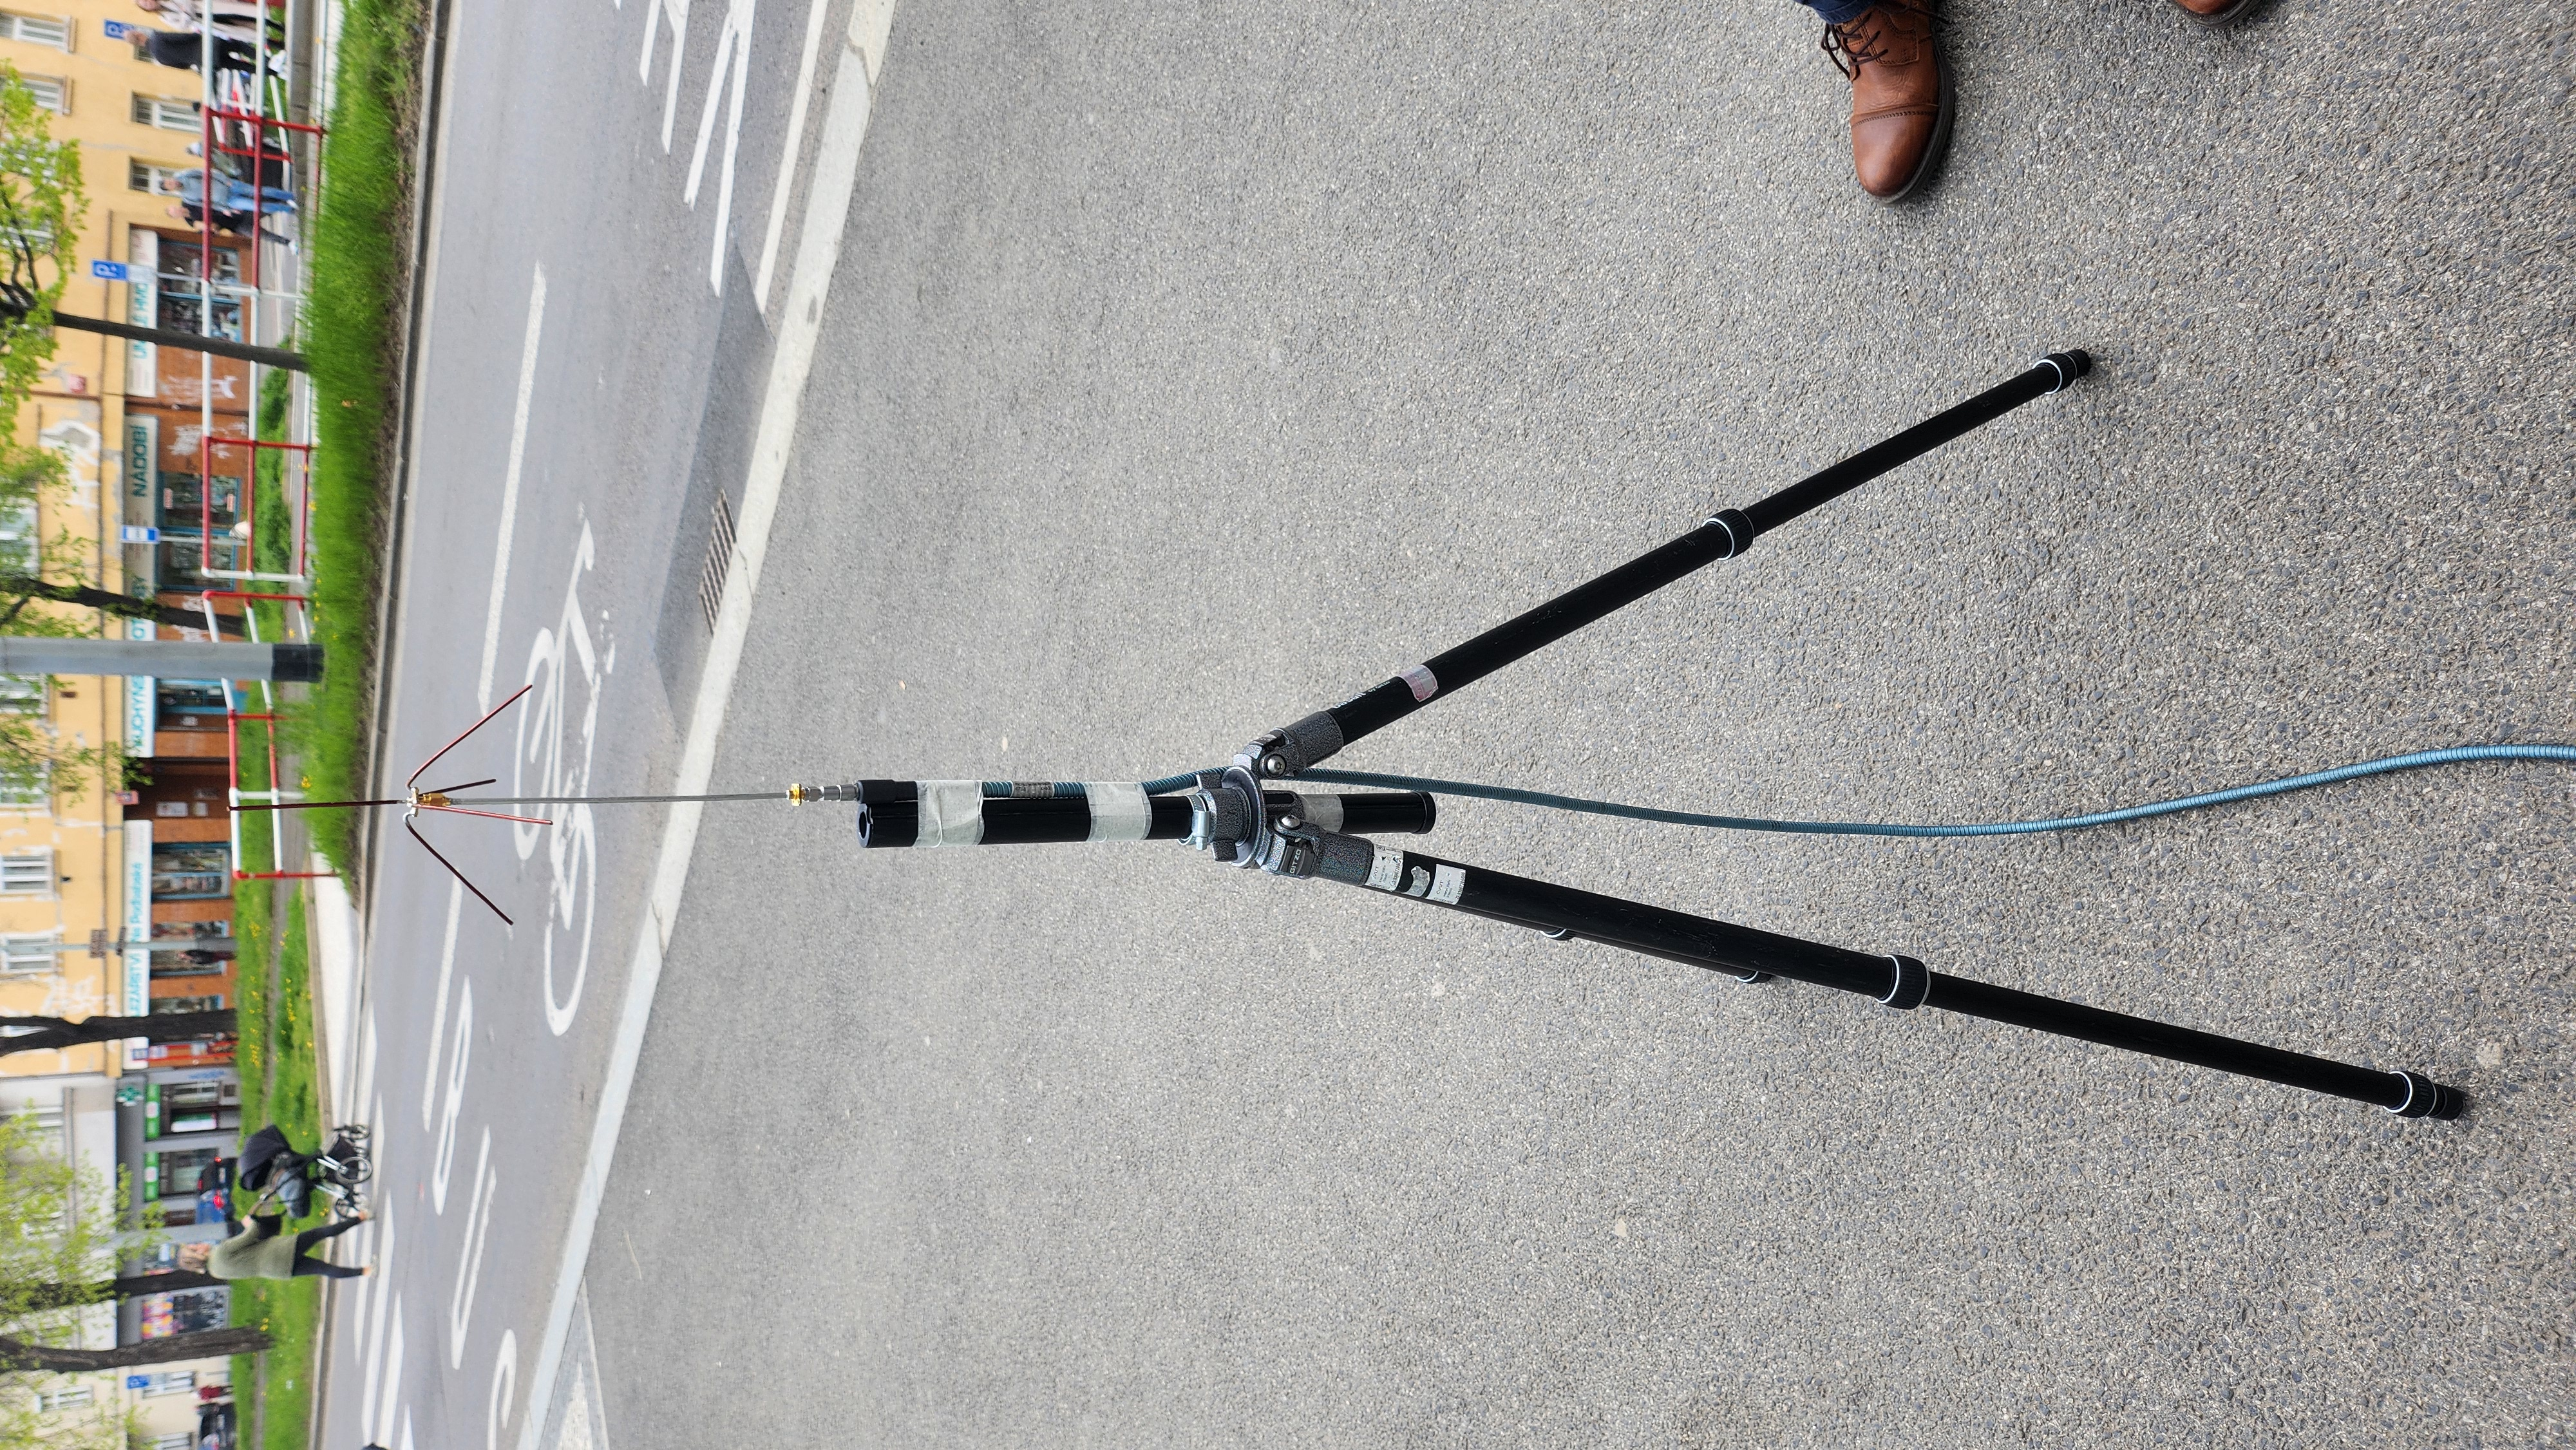
\includegraphics[angle=270,scale=0.08]{img/antenna_uniky_menza.jpg}
    \caption{Vysílací anténa umístěná vedle Technické Menzy bez zastínění}
    \label{fig:my_label}
\end{figure}

\begin{figure}[h!]
    \centering
    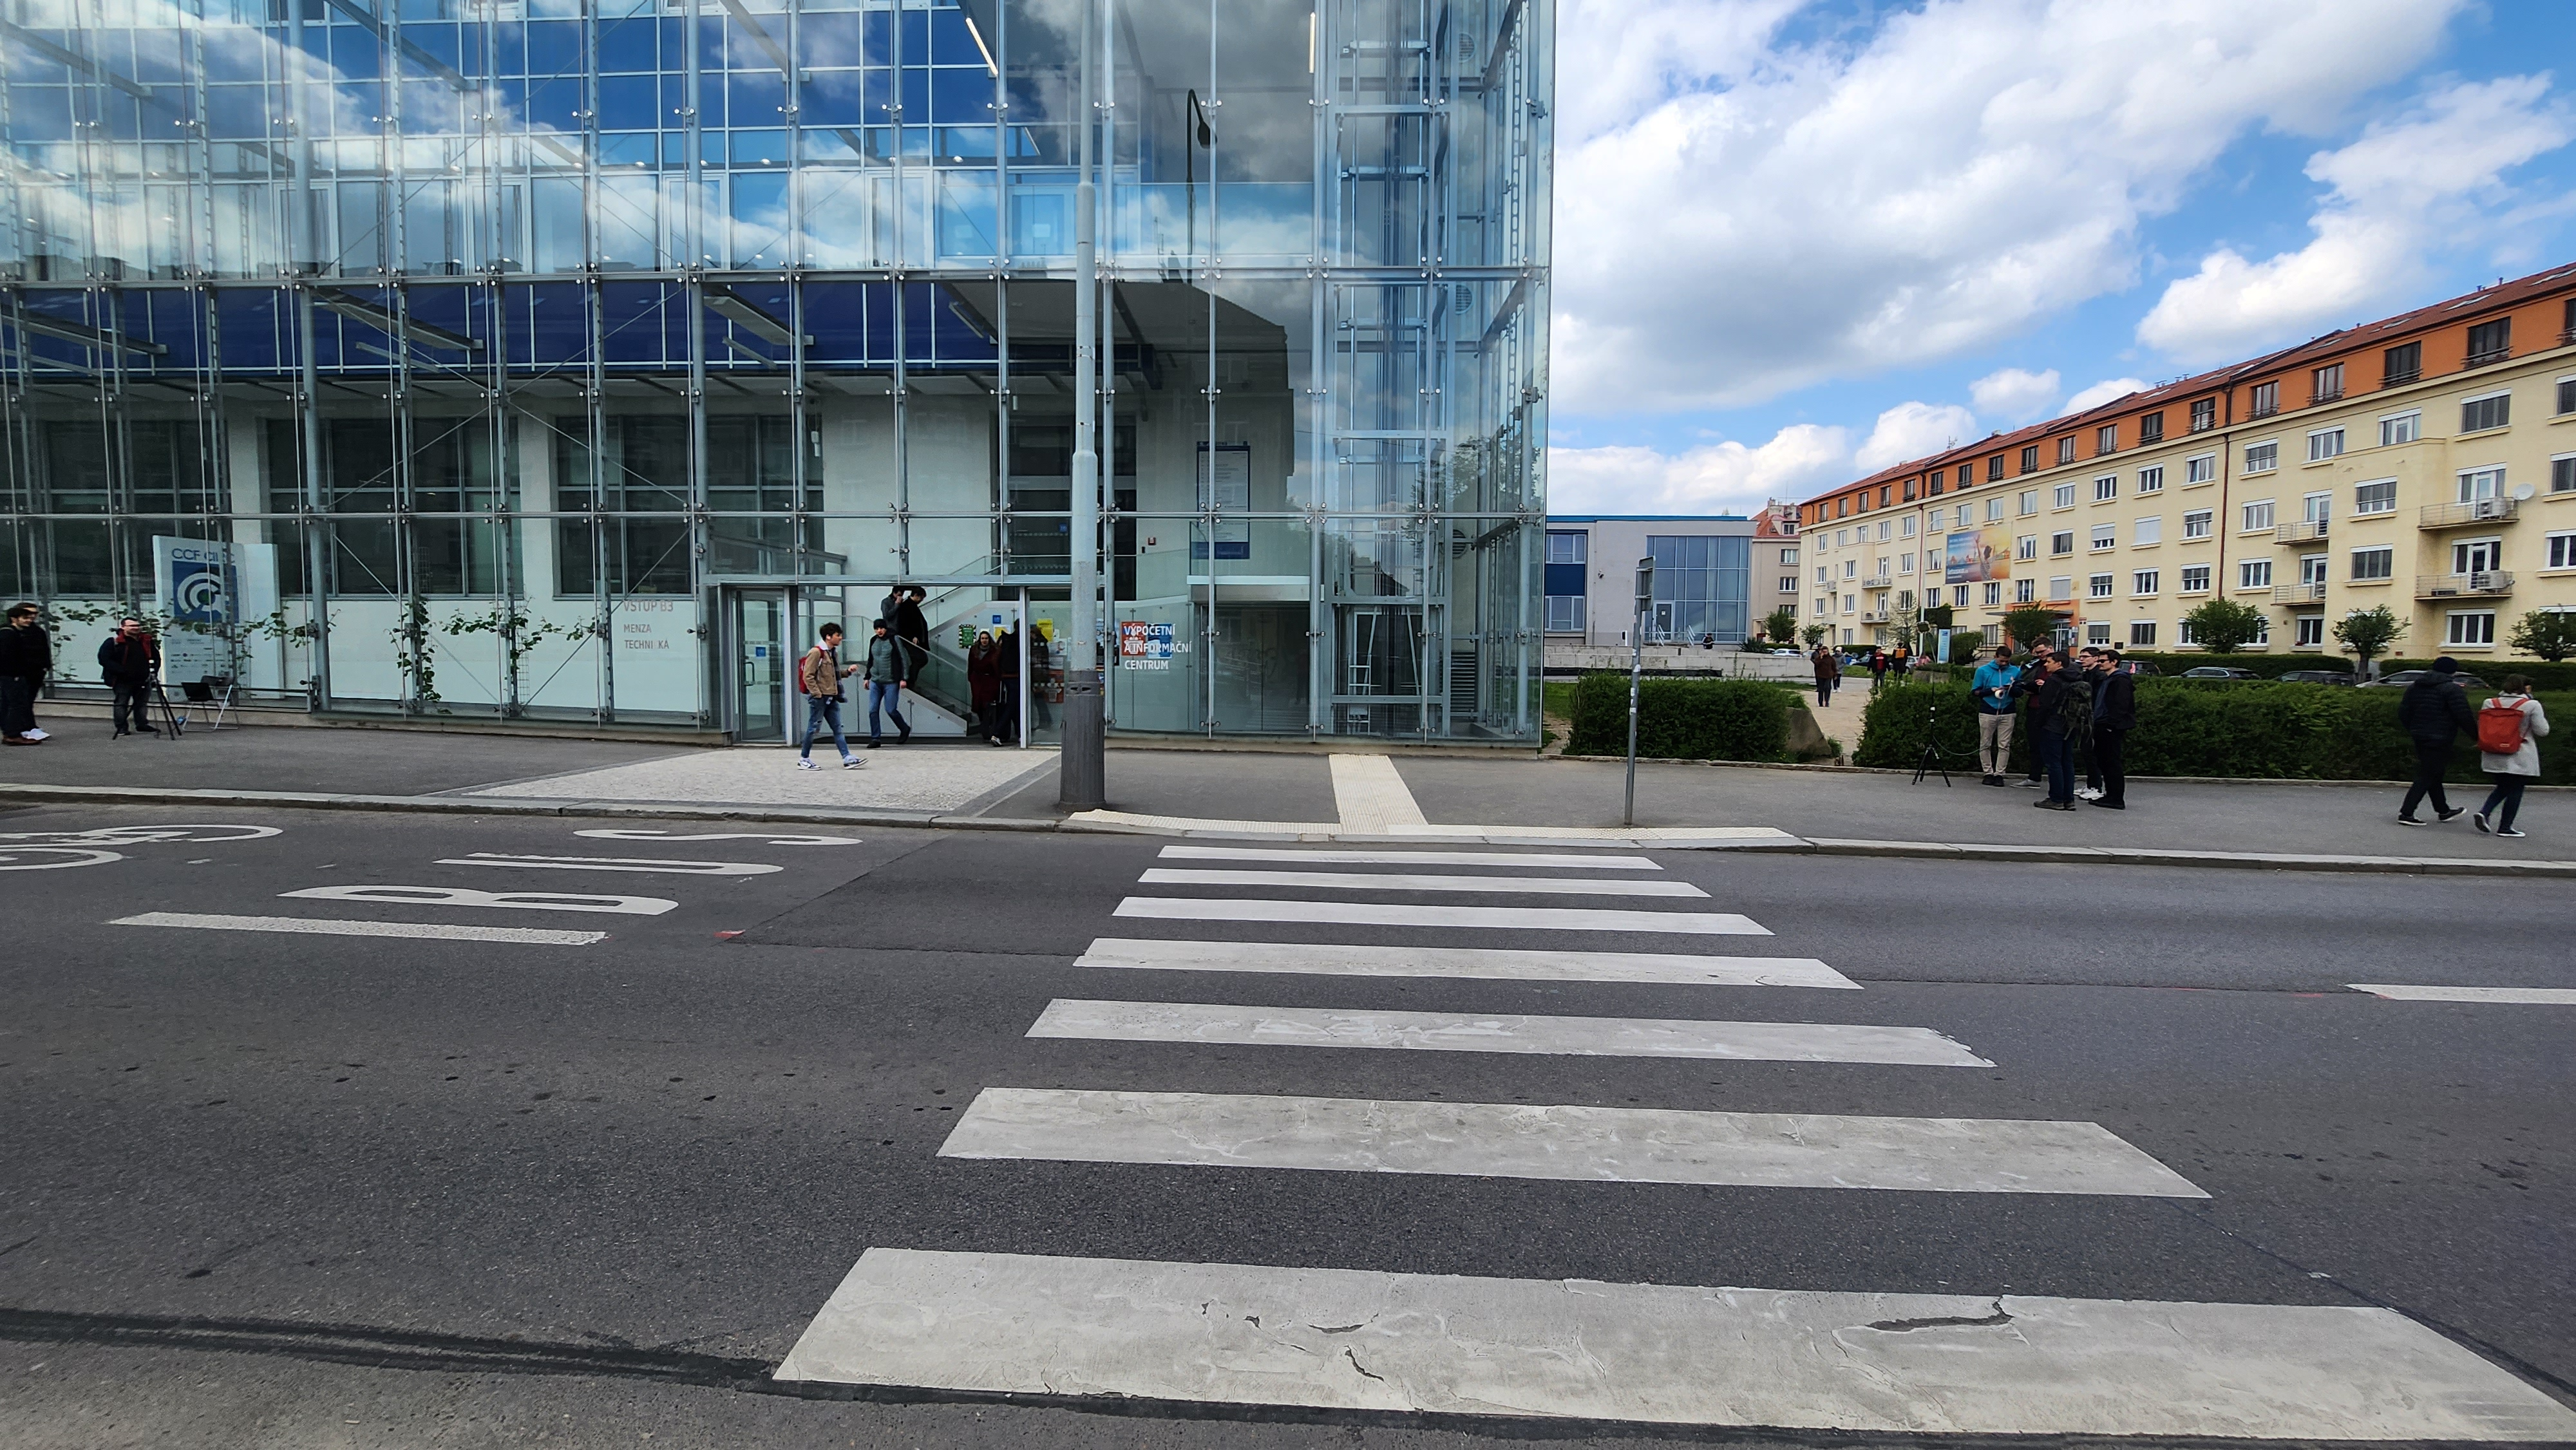
\includegraphics[,scale=0.1]{img/foto_uniky_menza.jpg}
    \caption{Fotka probíhajícího měření před Technickou menzou bez zastínění}
    \label{fig:my_label}
\end{figure}

\section{Měření bez zastínění}
Pro tento typ měření jsme se snažili najít vhodnou chvíli, kdy se mezi anténami nebude nikdo pohybovat. Bohužel se nám nepodařilo najít delší úsek, alespoň minutový, kdy by byly ideální podmínky.  Z toho důvodu jsme si vybrali několik různých časových úseků z delšího měření, které jsme poté spojili. Výsledné měření odpovídá očekávání, tedy celkový medián -64.5 dB. Po převedení dat na relativní úroveň vůči mediánu a vykreslení distribuční funkce, je při srovnání s teoretickou Rayleigho distribucí normovanou vůči mediánu je vidět, že tyto křivky se nekopírují, protože nedocházelo k zastínění.

\begin{table}[h!]
\centering
\begin{tabular}{|c|c|}
  \hline
   & RSS \\
  \hline
  Min & -77.06 dBm\\
  \hline
  Max & -56.19 dBm\\
  \hline
  Median & -64.5 dBm \\
  \hline
\end{tabular}
\caption{Tabulka maximální hodnoty, minimální hodnoty a medianu naměřených před Technickou menzou bez zastínění}
\end{table}

\begin{table}[h!]
\centering
\begin{tabular}{|c|c|}
  \hline
   Percentil &  \\
  \hline
  1 \% & -9.41 dB\\
  \hline
  10 \% & -5.39 dB\\
  \hline
  50 \% & 0 dB \\
  \hline 
  90 \% & 3.9 dB \\
  \hline
\end{tabular}
\caption{Tabulka percentilů z dat naměřených před Technickou menzou bez zastínění}
\end{table}

\clearpage

\begin{figure}[h!]
    \centering
    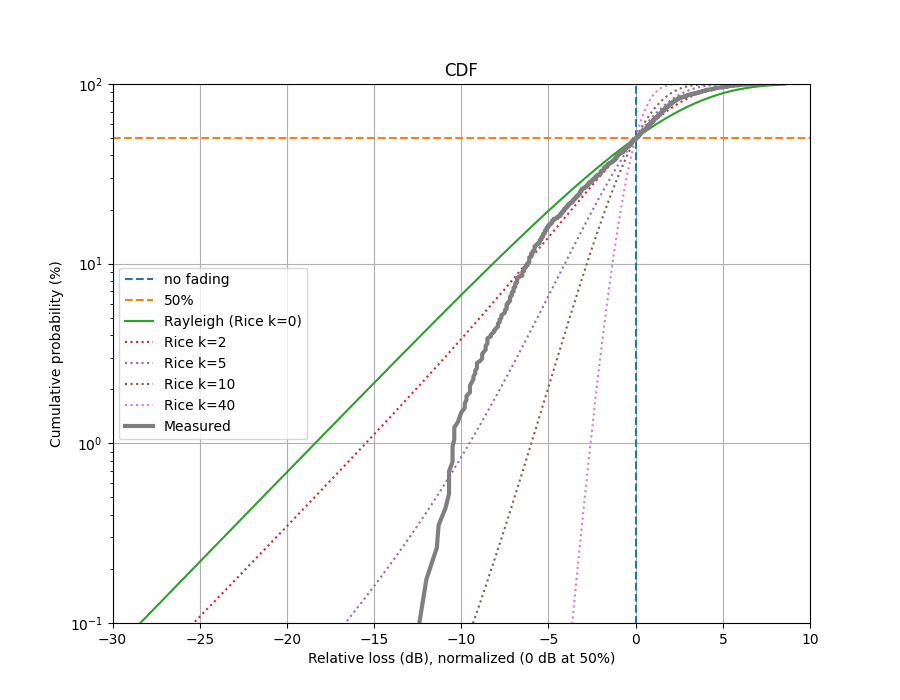
\includegraphics[,scale=0.64]{img/Static_scenario3.png}
    \caption{Distribuční funkce naměřených hodnot bez zastínění}
    \label{fig:my_label}
\end{figure}

\begin{figure}[h!]
    \centering
    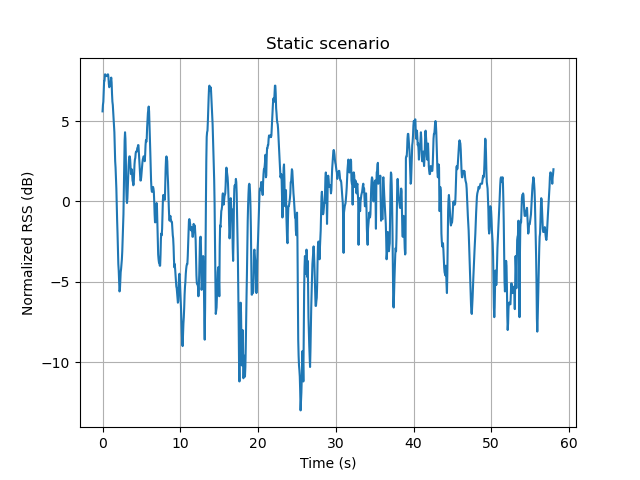
\includegraphics[,scale=0.85]{img/Static_scenario1.png}
    \caption{Naměřené hodnoty v čase bez zastínění, normalizované}
    \label{fig:my_label}
\end{figure}

\clearpage

\begin{figure}[h!]
    \centering
    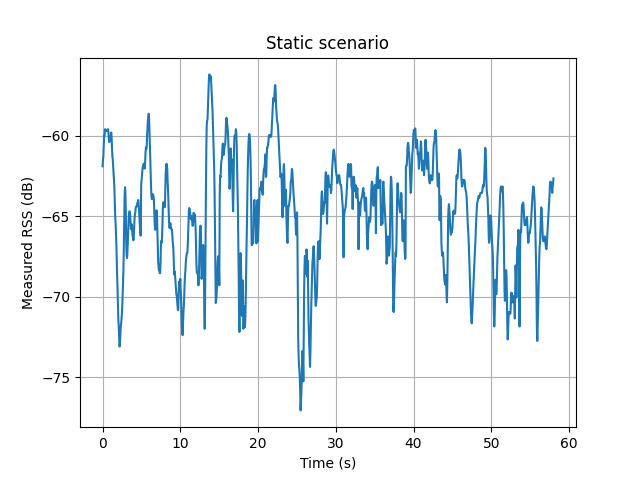
\includegraphics[,scale=0.85]{img/Static_scenario1_Measured.png}
    \caption{Naměřené hodnoty v čase}
    \label{fig:my_label}
\end{figure}

\section{Případ dynamického zastínění}
Pro tento typ měření jsme záměrně volili intervaly, kdy se budou mezi anténami pohybovat v dostatečném počtu lidé. Takový interval nebylo těžké nalézt, a to ani dokonce v dostatečně dlouhém časovém intervalu, který jsme si na začátku měření stanovili.
Celkový medián je -69.7 dB, útlum je tedy větší než v případě bez zastínění. Po převedení dat na relativní úroveň vůči mediánu a vykreslení distribuční funkce, je při srovnání s teoretickou Rayleigho distribucí normovanou vůči mediánu je vidět, že tyto dvě křivky už kopírují stejný trend, avšak ne dokonale, protože nedochází k úplnému zastínění po celou dobu měření.

\begin{table}[h!]
\centering
\begin{tabular}{|c|c|}
  \hline
   & RSS \\
  \hline
  Min & -93.1 dBm\\
  \hline
  Max & -61.0 dBm\\
  \hline
  Median & -69.7 dBm \\
  \hline
\end{tabular}
\caption{Tabulka maximální hodnoty, minimální hodnoty a medianu naměřených před Technickou menzou s dynamickým zastíněním}
\end{table}
\clearpage
\begin{table}[h!]
\centering
\begin{tabular}{|c|c|}
  \hline
   Percentil &  \\
  \hline
  1 \% & -15.5 dB\\
  \hline
  10 \% & -7.2 dB\\
  \hline
  50 \% & 0 dB \\
  \hline
  90 \% & 4.8 dB \\
  \hline
\end{tabular}
\caption{Tabulka percentilů z dat naměřených před Technickou menzou s dynamickým zastíněním}
\end{table}




%Obrazek - Distribuční funkce bez zastínění - DETAILNĚJŠÍ (druhou vymazat) A TU JEDNU NUTO OPRAVIT!!!
\begin{figure}[h!]
    \centering
    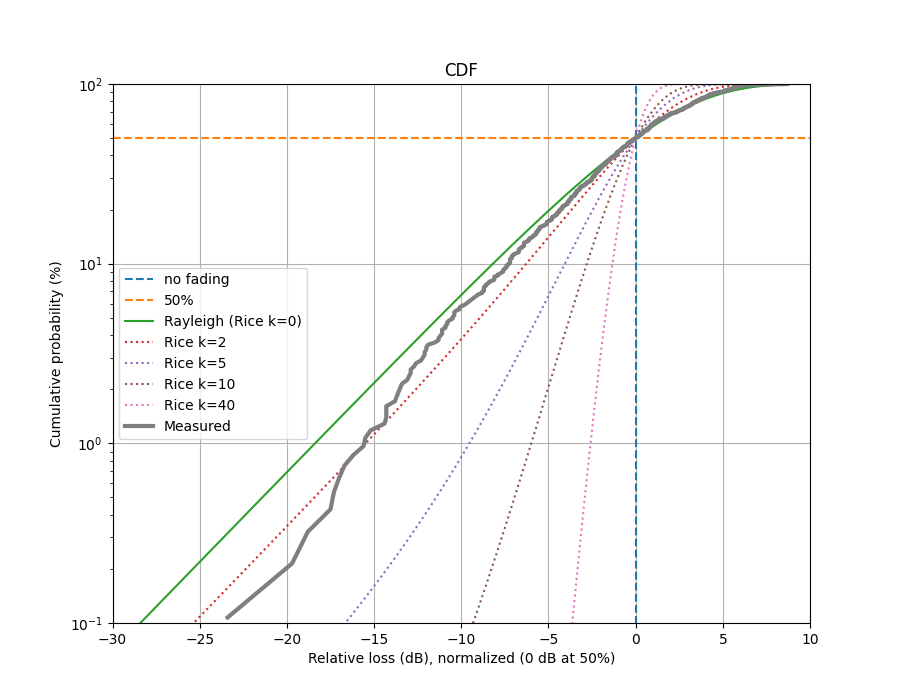
\includegraphics[,scale=0.6]{img/Crowd_scenario3.png}
    \caption{Distribuční funkce naměřených hodnot s dynamickým zastíněním}
    \label{fig:my_label}
\end{figure}
% Obrazek - normalikovane hodnoty v case - VYSTREDIT VUCI STREDNI HODNOTE
\clearpage
\begin{figure}[h!]
    \centering
    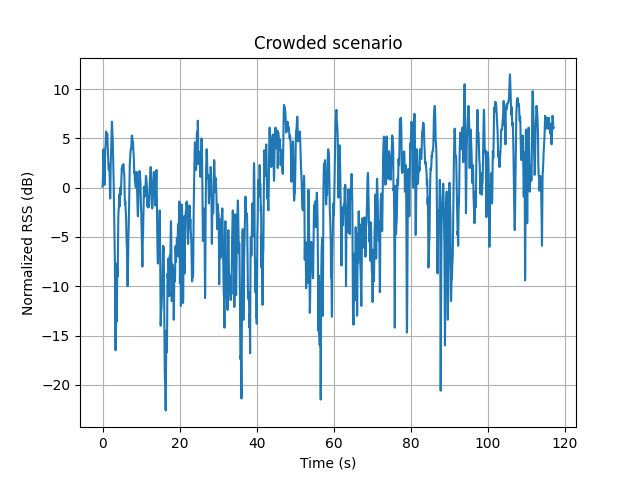
\includegraphics[,scale=0.85]{img/Crowd_scenario1.png}
    \caption{Naměřené hodnoty v čase s dynamickým zastíněním, normalizované}
    \label{fig:my_label}
\end{figure}

% Obrazek - nenormalizovaný ??????????????????? - STREDNI HODNOTA!!!
\begin{figure}[h!]
    \centering
    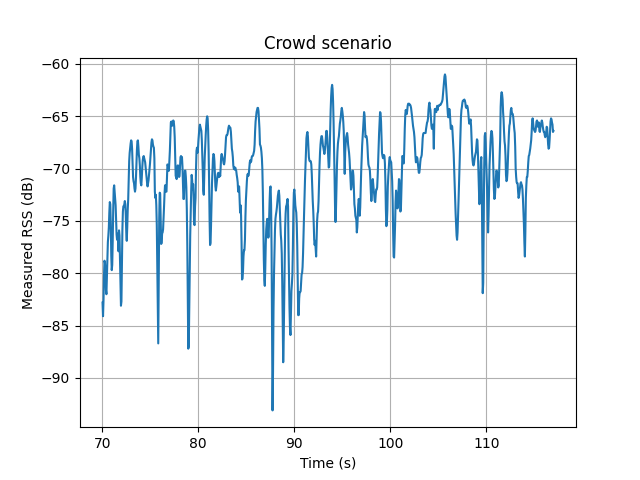
\includegraphics[,scale=0.85]{img/Crowd_scenario1_Measured.png}
    \caption{Naměřené hodnoty v čase s dynamickým zastíněním}
    \label{fig:my_label}
\end{figure}


\section{Případ úplného zastínění}
Při tomto scénáři jsme se snažili najít takový okamžik, kdy bylo co největší zastínění mezi anténami. Největší zastínění se nám podařilo získat, když většina osob procházela dveřmi do menzy. Navíc, my jako členové týmu jsme se pohybovali mezi anténami pro zvýšení efektu. Bohužel se nám nepodařilo zachytit dostatečně dlouhý úsek, kdy by došlo k úplnému zastínění. Z toho důvodu jsme vybrali z měření kratší úsek, který byl pro další analýzu vložen vícekrát za sebe. Tím dojde alespoň k vyhlazení křivky. Kolega, který nás měl na starost, nám sám řekl, že v tomto scénáři je úplné zastínění velice těžko proveditelné, ač jsme se snažili sebevíce. Proto jsme alespoň zkusili analyzovat následující krátký úsek měření, než tuto část úplně vynechat. 
Celkový medián je -78.4 dB. Po převedení dat na relativní úroveň vůči mediánu a vykreslení distribuční funkce, je při srovnání s teoretickou Rayleigho distribucí normovanou vůči mediánu vidět že křivka nekopíruje Rayleigho distribuční funkci, protože nedocházelo k úplnému zastínění.

\begin{table}[h!]
\centering
\begin{tabular}{|c|c|}
  \hline
   & RSS \\
  \hline
  Min & -93.1 dBm\\
  \hline
  Max & -65.5 dBm\\
  \hline
  Median & -78.4 dBm \\
  \hline
\end{tabular}
\caption{Tabulka maximální hodnoty, minimální hodnoty a medianu naměřených před Technickou menzou}
\end{table}



\begin{table}[h!]
\centering
\begin{tabular}{|c|c|}
  \hline
   Percentil &  \\
  \hline
  1 \% & -11.5 dB\\
  \hline
  10 \% & -6.7 dB\\
  \hline
  50 \% & 0 dB \\
  \hline1 
  90 \% & 5.6 dB \\
  \hline
\end{tabular}
\caption{Tabulka percentilů z dat naměřených před Technickou menzou}
\end{table}

\clearpage

%Obrazek - Distribuční funkce bez zastínění - DETAILNĚJŠÍ (druhou vymazat) A TU JEDNU NUTO OPRAVIT!!!
\begin{figure}[h!]
    \centering
    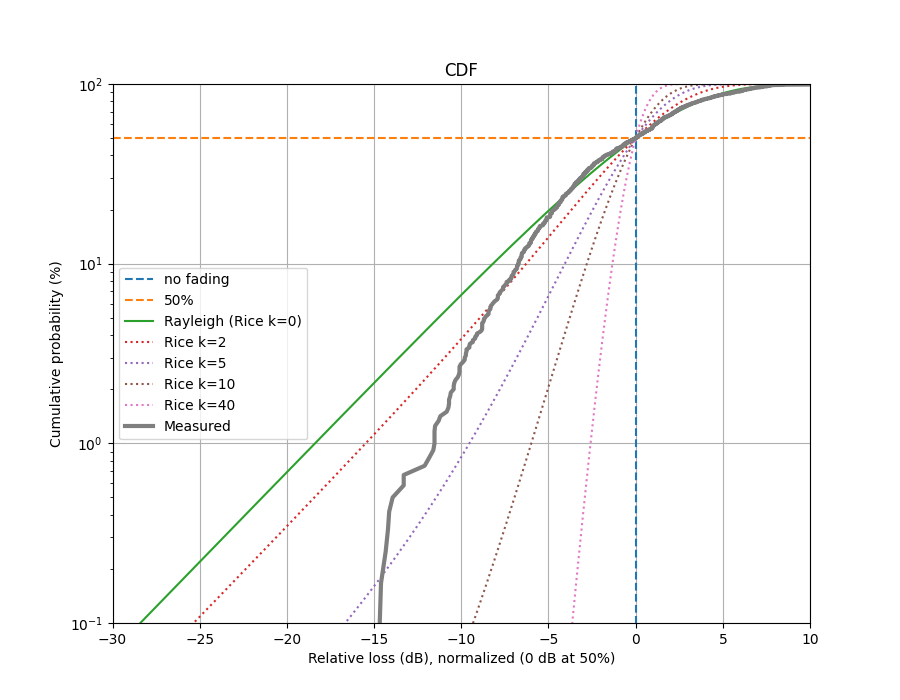
\includegraphics[,scale=0.62]{img/Dense_scenario3.png}
    \caption{Distribuční funkce naměřených hodnot s dynamickým zastíněním}
    \label{fig:my_label}
\end{figure}


% Obrazek - normalikovane hodnoty v case - VYSTREDIT VUCI STREDNI HODNOTE

\begin{figure}[h!]
    \centering
    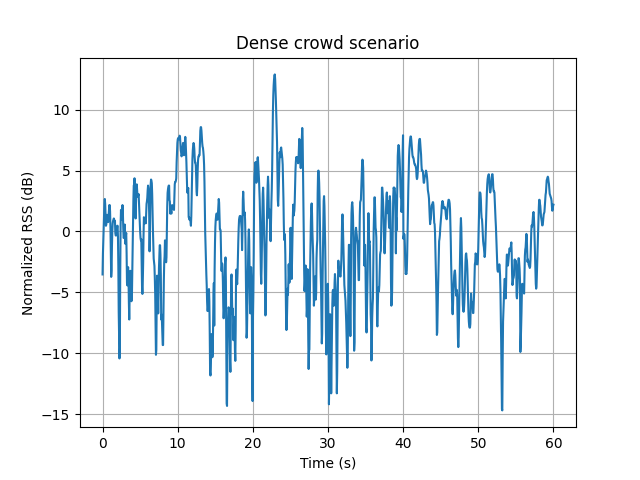
\includegraphics[,scale=0.82]{img/Dense_scenario1.png}
    \caption{Naměřené hodnoty v čase, normalizované}
    \label{fig:my_label}
\end{figure}
\clearpage
% Obrazek - nenormalizovaný ??????????????????? - STREDNI HODNOTA!!!
\begin{figure}[h!]
    \centering
    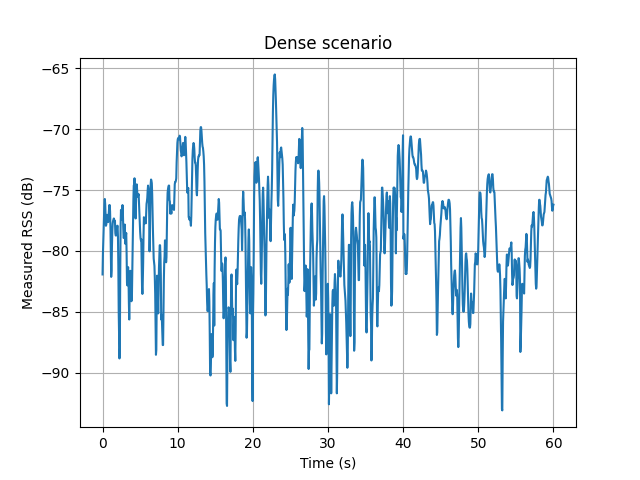
\includegraphics[,scale=0.85]{img/Dense_scenario1_Measured.png}
    \caption{Naměřené hodnoty v čase}
    \label{fig:my_label}
\end{figure}

\section{Shrnutí měření}
Při měření úniků jsme se snažili zachytit tři různé scénáře zastínění, konkrétně: bez zastínění, dynamické zastínění a úplné zastínění.
Při srovnání jednotlivých typů vůči Rayleigho distribuci je vidět, že pokus zachycení o úplného zastínění nevyšel, protože nekopíruje Rayleigho distribuci tak jak bychom čekali. 
V rámci měření dynamického a ne-zastínění lze pozorovat očekávaný trend.



